\documentclass[10pt]{standalone}

\usepackage[english]{babel}
\usepackage{amsmath,amsthm,amssymb,amsfonts}
\usepackage[italicdiff]{physics}
\usepackage[T1]{fontenc}
\usepackage{lmodern}
\usepackage[dvipsnames]{xcolor}
\usepackage[utf8]{inputenc}
\usepackage{tikz,tikz-3dplot,tikz-cd,pgf,pgfplots}
\usetikzlibrary{arrows.meta}
\pgfplotsset{compat=newest}

\setlength{\parindent}{0pt}

% Created August 7, 2021

\begin{document}

\thispagestyle{empty}

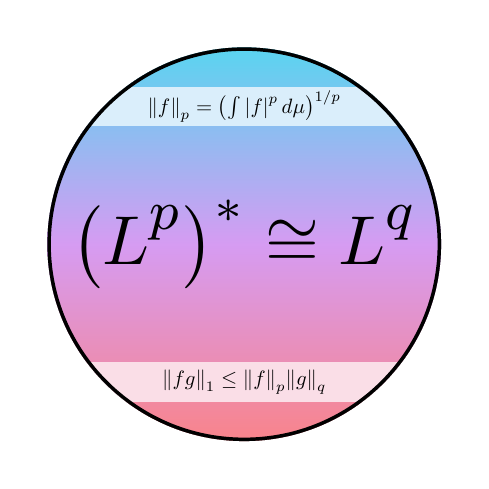
\begin{tikzpicture}[scale=2.5,every node/.style={transform shape}]
    \definecolor{tcol}{HTML}{12C2E9} % Top color
    \definecolor{mcol}{HTML}{C471ED} % Middle color
    \definecolor{bcol}{HTML}{F64F59} % Bottom color

    %%% Border for profile picture (to be cropped out)
    \clip (-1.1,-1.1) rectangle (1.1,1.1);

    %%% Interior and middle text
    \fill[very thick,top color=tcol!70,bottom color=bcol!70,middle color=mcol!70] (0,0) circle (1);
    \node at (0,0) {$\qty(L^{\raisebox{0.5mm}{\footnotesize\ensuremath p}})^*\cong L^{\raisebox{0.5mm}{\footnotesize\ensuremath q}}$};

    %%% Stripes and text within stripes
    \clip (0,0) circle (1); % Crop for stripes
    \fill[bcol!70!mcol!20] (-1,-0.8) rectangle (1,-0.6);
    \fill[tcol!70!mcol!20] (-1,0.6) rectangle (1,0.8);
    \node[scale=0.3] at (0,0.7) {$\norm{f}_p=\qty(\int\abs{f}^p\,d\mu)^{1/p}$};
    \node[scale=0.3] at (0,-0.7) {$\norm{fg}_1\le\norm{f}_p\norm{g}_q$};

    %%% Circle outline
    \draw[line width=2.5pt] (0,0) circle (1);
\end{tikzpicture}

\end{document}